\chapter{Appendices}


\section*{Appendix A: Gantt Chart}\vspace{-6em}
\begin{figure}[h!]
    \setlength{\abovecaptionskip}{-4em} 
    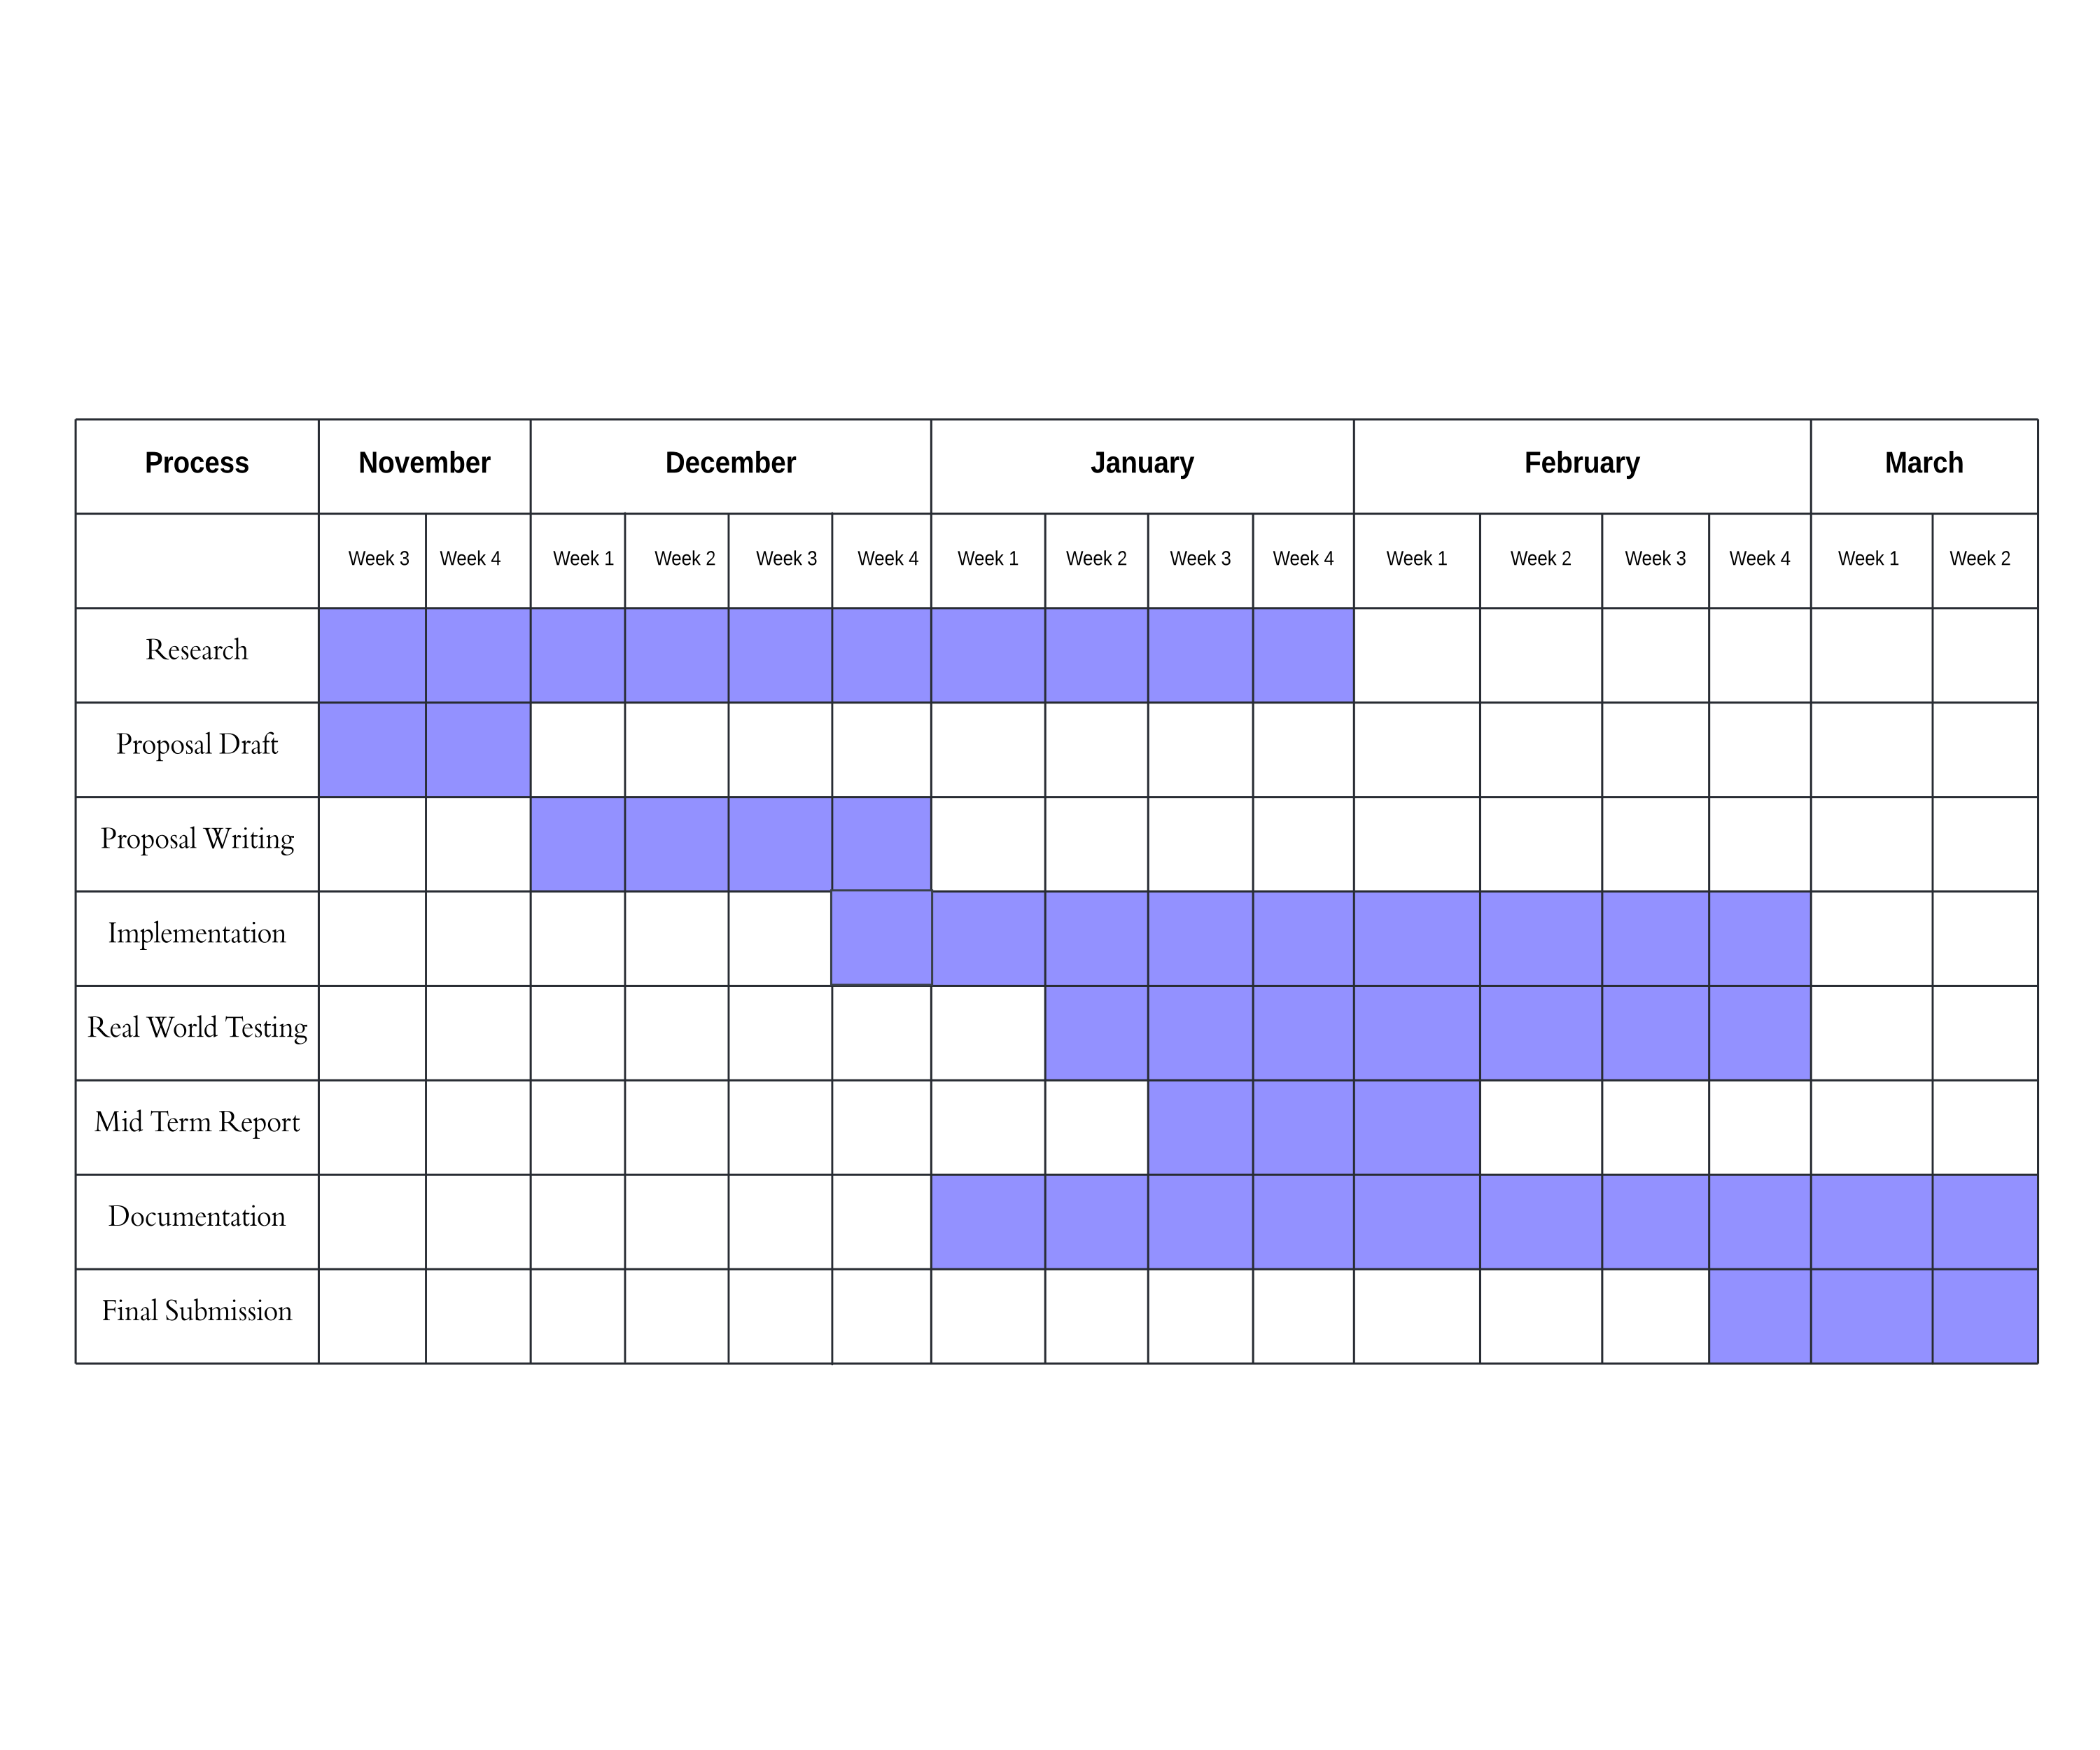
\includegraphics[width=\textwidth]{content/images/ganttChart.png}
    \caption{Project Timeline}
    \label{fig:gantt-chart}
\end{figure}
\newpage



\section*{Appendix B: Budget Estimation}
\begin{table}[h!]
    \centering
    \caption{Project Budget}
    \label{tab:budget-estimation}
    \begin{tabular}{|c|l|c|c|c|}
        \hline
        \textbf{S.N.} & \textbf{Components}                & \textbf{Quantity} & \textbf{Unit Price (NPR)} & \textbf{Total Price (NPR)} \\ \hline
        1  & Arduino                           & 1                  & 1500                      & 1500                       \\ \hline
        2  & ESP32-CAM                         & 1                  & 900                       & 900                        \\ \hline
        3  & Nema 17 Stepper Motor             & 1                  & 1500                      & 1500                       \\ \hline
        4  & A4988 Stepper Driver              & 1                  & 210                       & 210                        \\ \hline
        5  & 9g Servo                          & 3                  & 270                       & 810                        \\ \hline
        6  & Matrix Board                      & 3                  & 100                       & 300                        \\ \hline
        7  & Lamination Sheets                 & 10                 & 10                        & 100                        \\ \hline
        8  & Display                           & 1                  & 250                       & 250                        \\ \hline
        9  & Buttons                           & 3                  & 10                        & 30                         \\ \hline
        10 & 7805 5V Regulator                 & 2                  & 15                        & 30                         \\ \hline
        11 & AMS1117 3.3V Regulator            & 1                  & 10                        & 10                         \\ \hline
        12 & Capacitors and Resistors          & 2 + 6              & 5                         & 40                         \\ \hline
        13 & 12V Adapter                       & 1                  & 300                       & 300                        \\ \hline
        14 & CNY70 IR Sensor                   & 3                  & 69                        & 207                        \\ \hline
        \textbf{Total} &                             &                    &                           & \textbf{6187}              \\ \hline
    \end{tabular}
\end{table}
\newpage

\section*{Appendix C: Detailed Component Specifications}
\begin{itemize}
    \item Arduino: 16MHz clock speed, 54 digital I/O pins, 16 analog inputs, 4 UARTs, 6 PWM outputs, 1 USB connection, and power jack.
    \item ESP32-CAM: Wi-Fi and Bluetooth functionality, 2MP camera with OV2640, 520MHz dual-core processor, supports up to 16MB of flash memory.
    \item Nema 17 Stepper Motor: 1.8° step angle, 12V rated voltage, holding torque 40N·cm, stepper motor type, typically used in 3D printers.
    \item A4988 Stepper Driver: Full-step, half-step, and microstep operation modes, adjustable current control, thermal shutdown and overload protection.
    \item 9g Servo: Continuous rotation, torque 2.5kg.cm, operating voltage 4.8V to 6.0V, with a speed of 0.12s/60°.
    \item Matrix Board: Breadboard with a 400 tie-points capacity, ideal for prototyping.
    \item Lamination Sheets: A4 size, standard thickness for memory cells.
    \item Display: 16x2 LCD Display, used for displaying text and information, operates on 5V, with a built-in controller.
    \item Buttons: Pushbutton switches, rated for 50,000 cycles, typically used for user inputs.
    \item 7805 5V Regulator: Output voltage 5V, output current up to 1A, used to regulate input voltages to a stable 5V for powering logic circuits.
    \item AMS1117 3.3V Regulator: Output voltage 3.3V, output current up to 800mA, widely used in low power applications.
    \item Capacitors and Resistors: Capacitors for voltage regulator, resistors for current limiting and voltage division.
    \item 12V Adapter: 12V DC output, typically used to power high-voltage components such as motors and sensors.
    \item CNY70 IR Sensor: Reflective optical sensor, with phototransistor output, used for optoelectronic scanning.
\end{itemize}



